% Low-level handoff timing, styled after Figure 2.1.
% Only the controller-facing signals are shown.
\begingroup
\sffamily
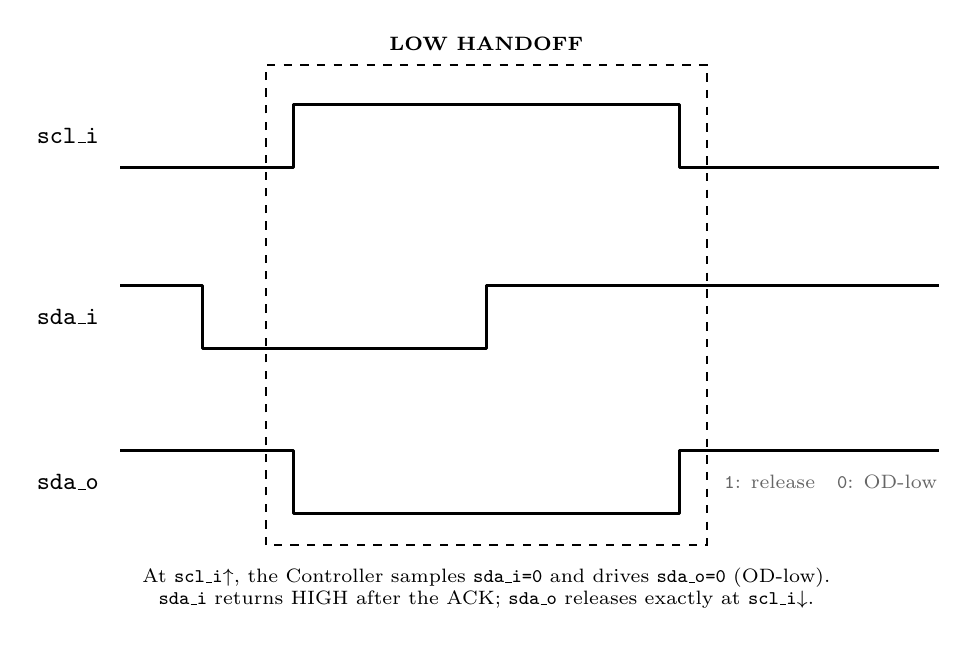
\begin{tikzpicture}[
    font=\small,
    wave/.style={draw=black, line width=1pt, line join=round},
    window/.style={draw=black, dashed, line width=0.6pt},
    siglabel/.style={font=\small\bfseries, anchor=east},
    condlabel/.style={align=center, font=\scriptsize\bfseries, text=black},
    note/.style={align=center, font=\scriptsize, text=black},
  ]

  % Handoff window: sample at SCL rising edge, release at falling edge.
  \draw[window] (1.85,0.55) rectangle (7.45,6.65);

  % scl_i: ACK/T-bit high phase is bounded by the rising/falling edges.
  \draw[wave]
    (0,5.35) -- (2.20,5.35) -- (2.20,6.15)
    -- (7.10,6.15) -- (7.10,5.35) -- (10.40,5.35);

  % sda_i: ACK is LOW briefly, then returns HIGH during SCL high.
  \draw[wave]
    (0,3.85) -- (1.05,3.85) -- (1.05,3.05)
    -- (4.65,3.05) -- (4.65,3.85) -- (10.40,3.85);

  % sda_o: Controller holds LOW through SCL high and releases at SCL falling.
  \draw[wave]
    (0,1.75) -- (2.20,1.75) -- (2.20,0.95)
    -- (7.10,0.95) -- (7.10,1.75) -- (10.40,1.75);

  \node[siglabel] at (-0.15,5.75) {\texttt{scl\_i}};
  \node[siglabel] at (-0.15,3.45) {\texttt{sda\_i}};
  \node[siglabel] at (-0.15,1.35) {\texttt{sda\_o}};

  \node[condlabel] at (4.65,6.92) {LOW HANDOFF};
  \node[note, anchor=north, text width=8.8cm] at (4.65,0.38)
    {At \texttt{scl\_i}$\uparrow$, the Controller samples \texttt{sda\_i=0} and drives
     \texttt{sda\_o=0} (OD-low). \texttt{sda\_i} returns HIGH after the ACK;
     \texttt{sda\_o} releases exactly at \texttt{scl\_i}$\downarrow$.};

  \node[note, anchor=west, text=black!60] at (7.55,1.35)
    {\texttt{1}: release\quad \texttt{0}: OD-low};
\end{tikzpicture}
\endgroup
